\chapter{Case study}
This chapter presents a case study where the load forecasting system is applied to Bruny Island.
As discussed in section \ref{scope} (\nameref{scope}), the aim of this case study is to develop a load forecasting system which can predict future load based on weather, holiday periods, car movement, and other factors. 
Bruny Island and the NAC will be used as a case study. 
The forecasting system will be equally applicable to any power system network, \hl{and this will be demonstrated later in this chapter}.
\\
Specifically, the system will have the following properties:
\begin{itemize}
	\item The system will produce a forecast up to 24 hours in the future in 15- to 60-minute intervals. This will be a rolling forecast that can be re-calculated at any time.
	\item The forecast will be able to begin from any point time.
	\item The forecast will predict load in kVA at each interval.
	\item The forecast system will be aimed at predicting aggregate load at the feeder level. That is, between approximately 0.5 and 10MVA.
	\item The forecast system will be especially tuned to predict load during holiday periods.
\end{itemize}

\begin{figure}
	\centering
	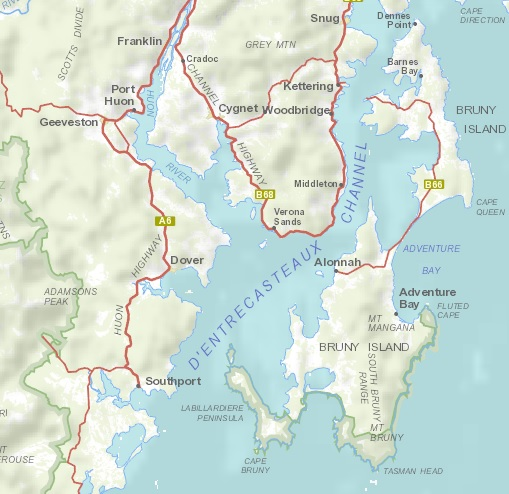
\includegraphics[width=0.35\linewidth]{images/bruny-basic}
	\caption{Bruny Island, in southern Tasmania, Australia. TODO: make a map that has expanded views to show the location on world map. QGIS, perhaps.}
	\label{fig:bruny-basic}
\end{figure}


\section{Data analysis}
In section \ref{pattens-profiles} the general properties of load profiles and how they are influenced by exogenous factors was discussed. Now, these general properties will be investigated in depth for the particular feeder in the case study.
\par
let's begin by having a simple look at some load profiles from the island.
Figure \ref{fig:load-profiles} shows apparent power draw on Bruny Island over a winter week, a summer week, and over an entire year.
The two weeks were selected to avoid special days such as holidays and are representative of typical weeks.
Some observations are immediately obvious
\begin{itemize}
	\item The midday load is only marginally larger than the overnight load in summer, but in winter it is significantly larger.
	\item Morning peaks are larger than afternoon peaks in summer, but in winter they are approximately equal.
	\item Thursday midday of the summer week appears abnormally high - perhaps this is a special day.
	\item There is some bad data on Tuesday of the summer week, as well as some missing data throughout the year.
	\item Over the whole year there appears to be a trend of increased max daily load over winter, which coincides with colder weather.
	\item There are some periods of abnormally large load over the year: March 27, June 11, and December 28.
\end{itemize}

\begin{figure}[htbp]
	\centering
	\subfigure[Apparent power delivered to Bruny Island over a single summer week]{
		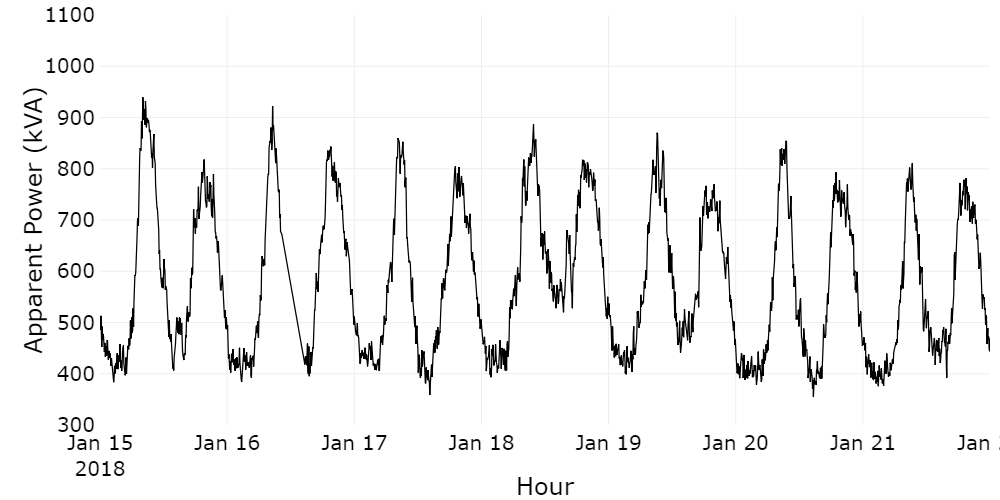
\includegraphics[width=.7\textwidth]{images/simple-week-summer}
		\label{fig:simple-week-summer}}
	\vfil
	\subfigure[Apparent power delivered to Bruny Island over a single winter week]{
		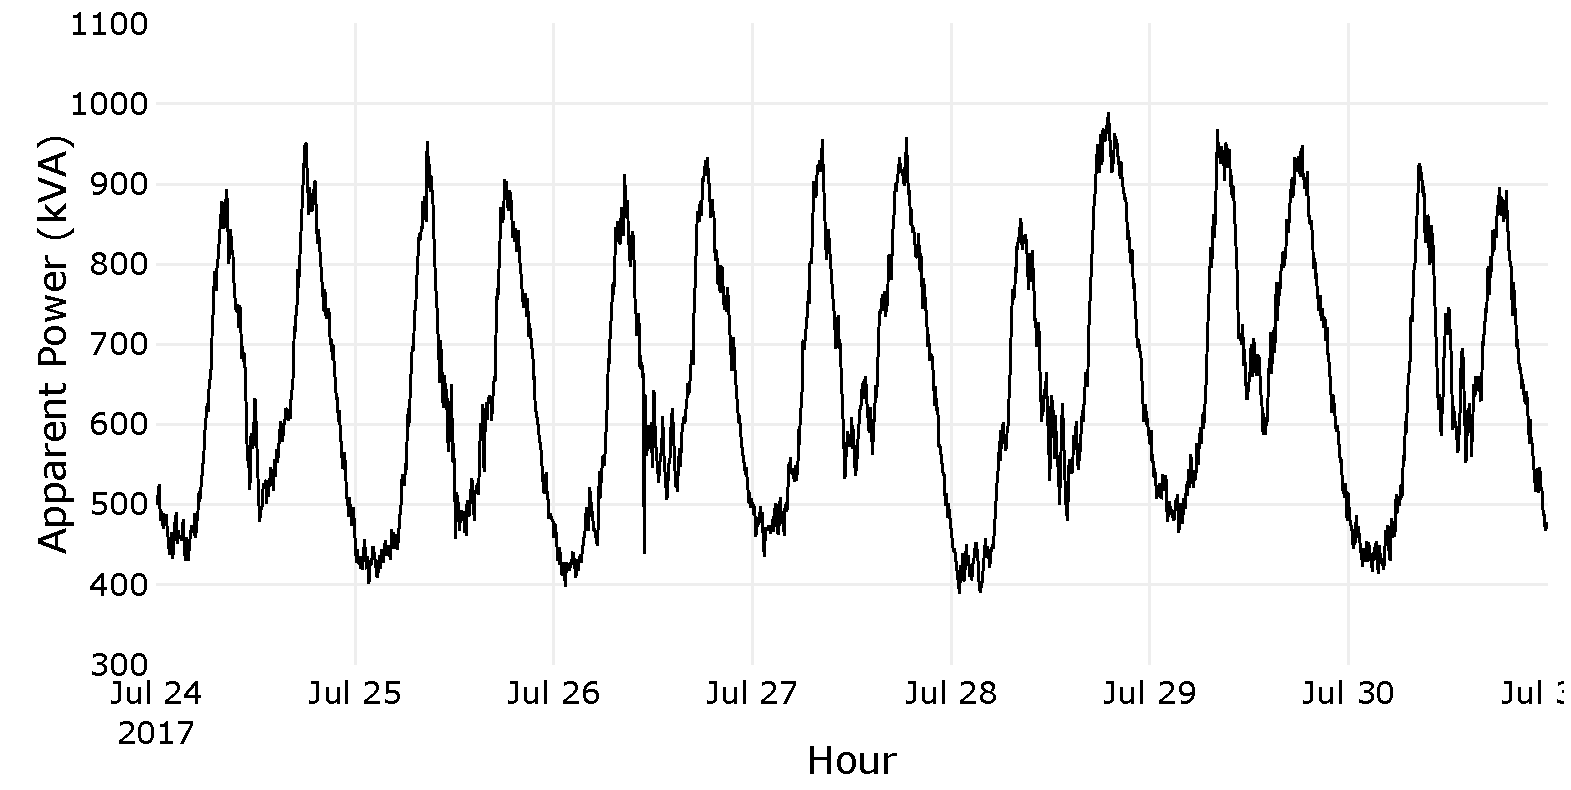
\includegraphics[width=.7\textwidth]{images/simple-week-winter}
		\label{fig:simple-week-winter}}
	\vfil
	\subfigure[Max load and temperature oer 2017]{
		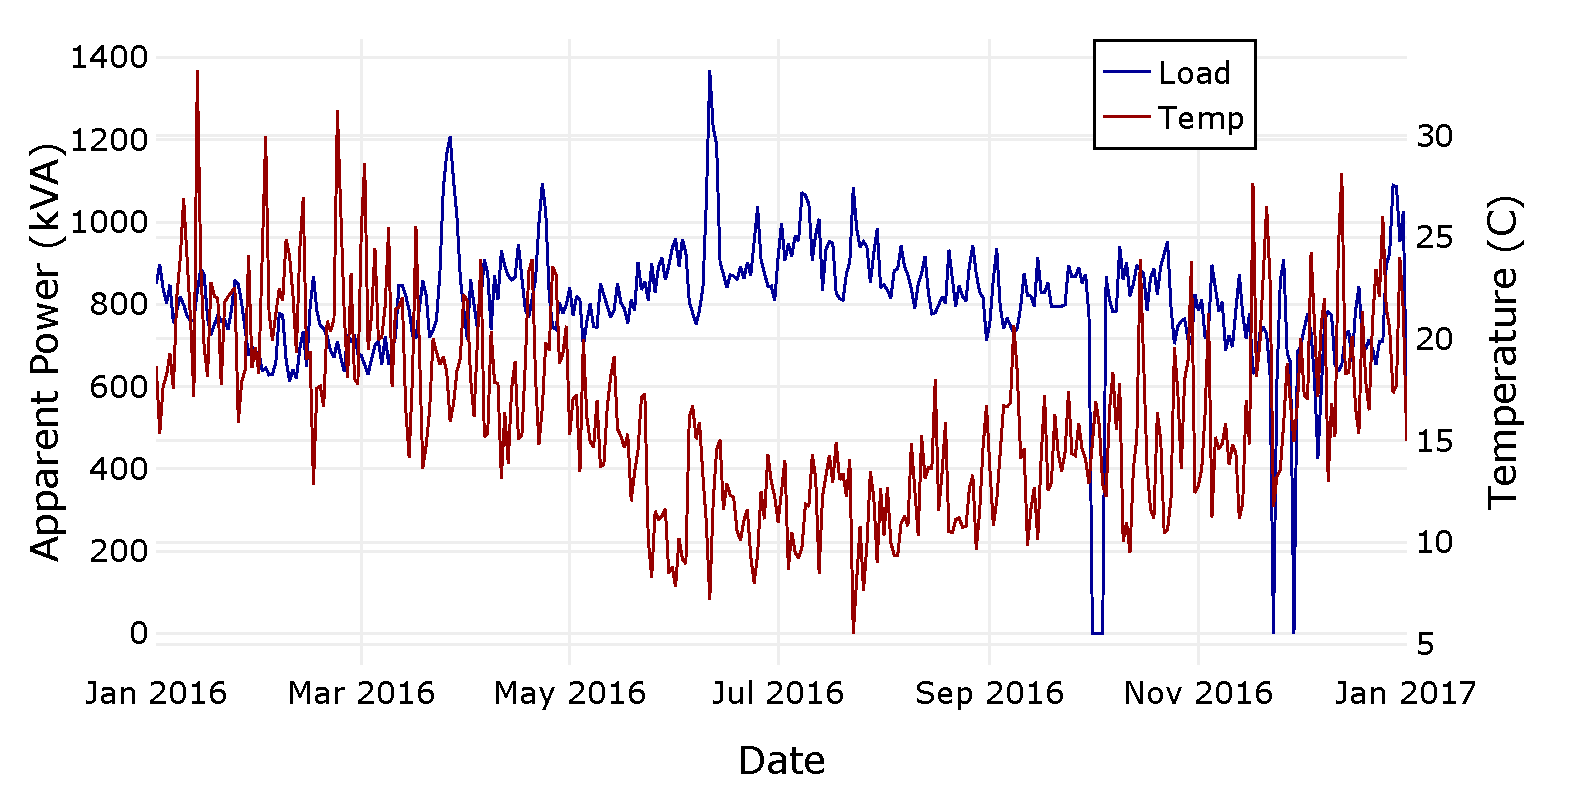
\includegraphics[width=.7\textwidth]{images/max-load-max-temp}
		\label{fig:max-load-max-temp}}
	\caption{Bruny Island load profiles}
	\label{fig:load-profiles}
\end{figure}

